\documentclass[10pt,letterpaper,twocolumn]{article}
\usepackage[T1]{fontenc}
\usepackage{lmodern}
\usepackage[letterpaper,top=0.60in,bottom=0.56in,left=0.70in,right=0.70in,columnsep=0.28in]{geometry}
\usepackage{graphicx,amsmath,booktabs,tabularx,xcolor,microtype,etoolbox}
\usepackage[hidelinks]{hyperref}
\usepackage{caption}
\captionsetup{font=small,labelfont=bf}
\apptocmd{\thebibliography}{\setlength{\itemsep}{1pt}\setlength{\parskip}{0pt}}{}{}
\definecolor{ink}{HTML}{23324D}
\definecolor{softblue}{HTML}{EEF2F7}
\definecolor{rust}{HTML}{984830}
\hypersetup{pdftitle={Scene-gated face detection on a wearable microcontroller},
  pdfauthor={Omri Steinberg-Tatman and Sophia Yuan},
  colorlinks=true,urlcolor=rust,linkcolor=ink,citecolor=rust}
\raggedbottom
\setlength{\parskip}{0pt}
\setlength{\parindent}{1em}
\setlength{\emergencystretch}{1em}
\setlength{\textfloatsep}{10pt plus 3pt minus 2pt}
\setlength{\dbltextfloatsep}{11pt plus 3pt minus 2pt}
\setlength{\floatsep}{10pt plus 3pt minus 2pt}
\renewcommand{\topfraction}{0.92}
\renewcommand{\dbltopfraction}{0.91}
\renewcommand{\textfraction}{0.07}
\newcommand{\stage}[2]{\colorbox{softblue}{\parbox[c][2.35em][c]{0.15\linewidth}{\centering\small\textbf{#1}\\[-1pt]\footnotesize #2}}}
\newcommand{\nextstage}{\hspace{0.55em}\textcolor{rust}{$\rightarrow$}\hspace{0.55em}}
\title{\vspace{-1.7em}\textbf{Scene-gated face detection on a wearable microcontroller}\\[-1pt]
{\large A paired power and latency study on the Arduino Nicla Vision}}
\author{Omri Steinberg-Tatman \and Sophia Yuan}
\date{\small UCLA ECE M202A / CS M213A \quad Fall 2026 \quad Project P04}
\begin{document}
\maketitle

\begin{abstract}
A wearable camera can keep processing nearly identical frames between encounters. We implemented a scheduler that leaves the camera running and calls a face detector when grayscale scene statistics change or a periodic check is due. We compared scene-gated and fixed processing on one Arduino Nicla Vision using ten independent power cycles and the same 29-second optical replay in each condition. Mean USB input power fell from 680.29 to 630.75\,mW, a paired saving of 49.54\,mW (7.28\%, 95\% confidence interval 46.97--52.12\,mW). Both policies localized the same 30 of 40 scripted face episodes and missed the far-outdoor episode on every replay. Median time to first matched detection rose from 0.65 to 1.38\,s among matched episodes. The gated policy made 68\% fewer detector calls. A separate USB test verified one saved photo per portrait encounter. The power result characterizes the tested board, meter, and replay, and the identity stage ran with known-person acceptance disabled.
\end{abstract}
\par\noindent\textbf{Keywords:} embedded vision, adaptive inference, face detection, power measurement

\section{Introduction}
A small camera often observes a static background for longer than it observes a face. A fixed processing cadence gives consistent opportunities to detect a new encounter, but it also repeatedly pays for detection during quiet intervals. A camera that first checks for changes in the image can spend less time running the detector. Global statistics can also miss subtle changes, including a face that covers a small part of the frame. Whether the shortcut pays off depends on the power that stays in the capture path and the delay a missed trigger introduces.

We ask whether a scene-change policy can reduce \emph{board input power} while preserving the same face episodes as a fixed policy on a repeatable workload. We measure elapsed time to the first localized face and include stage controls to explain the power difference. The original proposal included recognizing a small enrolled group. Our compact models ran on the device, but crop benchmarks showed weak correct acceptance, so we used the stated adaptive face-detection fallback. The project contributed an on-device scheduler, a paired power and response study with raw-packet replay, and a USB demo that saves one image per detected encounter.

\section{Related work}
NoScope couples difference detectors with specialized networks to avoid unnecessary video-query inference \cite{noscope}. Our scheduler uses grayscale statistics as a lightweight trigger before a single shared detector. ADMN adjusts compute across modalities and layers in response to input quality and resource constraints \cite{admn}. Our case keeps one camera active and changes the schedule of detector calls. Viola and Jones introduced the cascaded Haar-feature method underlying the native detector \cite{viola}. MobileNetV1 motivates the depthwise separable architecture of the small embedding model \cite{mobilenet}. QMUL-SurvFace provides low-resolution surveillance crops for the separate host recognition study \cite{survface}.

We contribute an on-device scheduler and its controlled evaluation, using an existing native detector and network architecture. NoScope's video-query throughput and ADMN's multimodal compute savings motivate adaptation, but their workloads and hardware do not provide directly comparable power baselines.

\section{System design}
\subsection{Camera and inference path}
The Arduino Nicla Vision runs OpenMV on an STM32H747 microcontroller \cite{nicla,openmv}. Its GC2145 camera supplies a centered \(240\times240\) grayscale region from a QVGA frame. The native Haar detector produces a candidate face box. If the box yields a valid crop, the runtime resizes it to \(96\times96\) and can invoke a MobileNetV1-derived \(\alpha=0.10\) INT8 embedding model (64 output dimensions). The model file is 101{,}576 bytes. A separate load of this same model used a 43{,}008-byte tensor arena. Camera buffers and the rest of the runtime use additional memory. Known-person acceptance was disabled in the measured configuration.

\begin{figure*}[t]
\centering
\stage{Capture}{\(240\times240\) gray}\nextstage
\stage{Schedule}{fixed or gated}\nextstage
\stage{Detect}{native Haar}\nextstage
\stage{Crop}{\(96\times96\)}\nextstage
\stage{Embed}{INT8, 64-D}
\caption{R19 pipeline on the Nicla. The scheduling policy changes when the detector runs. A valid face crop is needed to reach the embedding stage. Linked camera frames and decisions can be viewed over USB.}
\label{fig:pipeline}
\end{figure*}

The USB host pairs each camera JPEG with a device result by boot ID, frame ID, and JPEG digest. The dashboard displays the matching frame, crop, and decision. With saving enabled, the host records one image per detected encounter and avoids duplicate saves while the face remains in view. The power study disabled photo saving to keep file writes out of the comparison.

\subsection{Scheduling policies}
Both policies use the same 250\,ms configured processing interval, camera settings, image-quality check, detector and embedding model. The camera remains awake, and the motion gate remains disabled. The fixed policy runs the detector on every eligible frame. The scene-gated policy computes absolute changes in the grayscale mean and standard deviation relative to the frame at the most recent detector call. A mean change of at least 8 intensity levels or a spread change of at least 6 triggers a check after a 500\,ms holdoff. The change latch clears once both differences return to 4 and 3 or less, respectively. The first eligible frame after startup or after roughly 2\,s without a detector call also triggers detection. A detector call refreshes the reference. The 2\,s period schedules eligibility checks, and actual execution still depends on frame availability and quality. This experiment changes execution timing; model precision, IR illumination, and sensor selection are outside the measured contrast.

\section{Evaluation}
\subsection{Bench and workload}
A fixed display replayed the 29-second \texttt{power-bodycam-v1} clip through the physical camera. Four scripted face segments alternate with four quiet intervals. The clip includes far outdoor, medium and near hallway, and a far segment with digital degradation that approximates a wet lens. This optical setup exercises the actual image sensor and firmware. The repeated clip controls exposure to the same scenes and gives a within-board comparison.

The USB supply path ran from a Windows laptop through a Belkin USB-C data hub and an FNIRSI C2 inline meter to the Nicla (Fig.~\ref{fig:bench}). A separate connection to the meter's PC/HID port logged voltage and current. Each accepted block included four workloads on the same R19 boot. Capture-only and detector-only controlled for the first two stages. The two full workloads ran the same detector and small embedding model using fixed or scene-gated scheduling. Physical power cuts yielded ten distinct board boot IDs with separate meter runs. Accepted schedule seeds were 62001--62007, 62009, 62010, and 62012. These identify trial orders, not additional people or training runs. The order of the two full pipelines was balanced across accepted blocks. Fixed went first five times.

\begin{figure}[t]
\centering
\setlength{\tabcolsep}{2pt}
\small
\begin{tabular}{@{}c@{}}
\colorbox{softblue}{\strut Windows host with Belkin USB-C hub}\\[3pt]
\textcolor{rust}{\(\downarrow\)}\enspace USB power and data\\[2pt]
\colorbox{softblue}{\strut FNIRSI C2 inline meter}\\[3pt]
\textcolor{rust}{\(\downarrow\)}\enspace Metered supply and serial\\[2pt]
\colorbox{softblue}{\strut Nicla Vision facing replay display}
\end{tabular}
\caption{Physical bench topology. The meter also had a separate HID logging cable to the Windows host. We cut power downstream of the meter between qualified blocks.}
\label{fig:bench}
\end{figure}

\subsection{Qualification and scoring}
Before and after each block, a checkerboard test verified optical alignment within a 3-pixel corner tolerance. Meter qualification required valid packet decoding, in-window sample values of 4.75--5.25\,V and 0.05--0.20\,A, and a maximum report gap of 200\,ms. Playback checks verified the intended clip and required UTC and monotonic boundaries to agree within 100\,ms. Frame-linkage checks required at least two linked observations per episode and 90\% linkage on the full inference workloads. The complete set of gates and tolerances is in the archive. All four windows had to pass qualification to include a block. The 20 accepted full-pipeline windows achieved 100\% preview linkage. Maximum accepted corner drift relative to the reference was 2.59 pixels. We kept the 28 excluded attempts in the ledger. They include preflight attempts, geometry failures, anomalous meter reports, and an interrupted video run.

The replay code averages the four voltage--current products in each accepted HID report, interpolates at the playback boundaries, and trapezoidally integrates power against exact host UTC receipt timestamps. It reproduced all 40 accepted windows to within \(4.0\times10^{-9}\) W of the saved window means. For block \(b\) and mode \(m\), we compute average input power \(\bar P_{b,m}=E_{b,m}/T_{b,m}\). The primary result is the mean of the ten paired savings,
\begin{equation*}
  d_b = \bar P_{b,\mathrm{fixed}} - \bar P_{b,\mathrm{gated}}, \qquad
  \bar d = \frac{1}{10}\sum_{b=1}^{10}d_b.
\end{equation*}
We report a two-sided, 95\% Student \(t\) interval across the ten block differences and divide \(\bar d\) by the fixed mean to report a percentage.

For face coverage, the camera-space annotation is projected from the source clip. A face episode counts as matched if at least one linked observation has a single predicted region whose intersection over union with that annotation reaches 0.30. Delay is measured from scripted episode onset to the first matched face box. We summarize medians among matched episodes. A model-stage match additionally requires crop coverage of at least 0.80 and completed inference. Detected faces in scripted quiet intervals are tabulated separately.

\section{Results}
\subsection{Input power}
\begin{table}[t]
\centering
\caption{Mean input power and observed energy. Each workload has ten accepted windows, with durations of 29.000--29.017\,s.}
\label{tab:power}
\small
\begin{tabular}{@{}lrr@{}}
\toprule
Workload & Power (mW) & Energy (J)\\
\midrule
Capture only & 608.72 & 17.66\\
Detector only & 670.17 & 19.44\\
Fixed pipeline & 680.29 & 19.73\\
Scene-gated pipeline & 630.75 & 18.30\\
\bottomrule
\end{tabular}
\end{table}

Scene gating reduced input power in all ten pairs (Fig.~\ref{fig:pairs}). Mean saving was 49.54\,mW (7.28\%) with a 95\% paired interval of 46.97--52.12\,mW. Individual savings ranged from 44.10 to 53.64\,mW. On a standardized 29-second interval, the power difference corresponds to 1.44\,J saved (95\% interval 1.36--1.51\,J). Table~\ref{tab:power} gives actual integrated energy means. The capture-only arm already drew 608.72\,mW and the detector-only arm drew 670.17\,mW. This helps explain why the drop in detector calls produced a smaller proportional reduction in total power (Fig.~\ref{fig:workloads}).

Savings averaged 46.51\,mW with fixed inference first and 52.58\,mW with gated inference first (five starts each). Both orders favored gating; this exploratory split suggests possible order effects.

\begin{figure}[t]
\centering
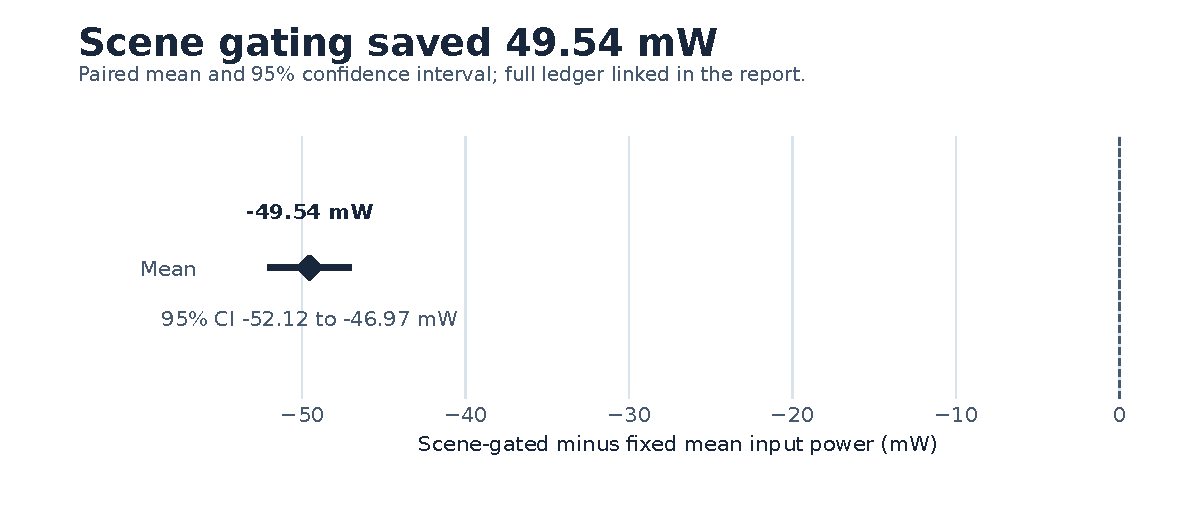
\includegraphics[width=\linewidth]{figures/01_paired_power.pdf}
\caption{Paired reduction in mean USB input power across ten physical starts. Markers distinguish which full pipeline ran first. The aggregate shows the paired 95\% interval.}
\label{fig:pairs}
\end{figure}

\begin{figure}[t]
\centering
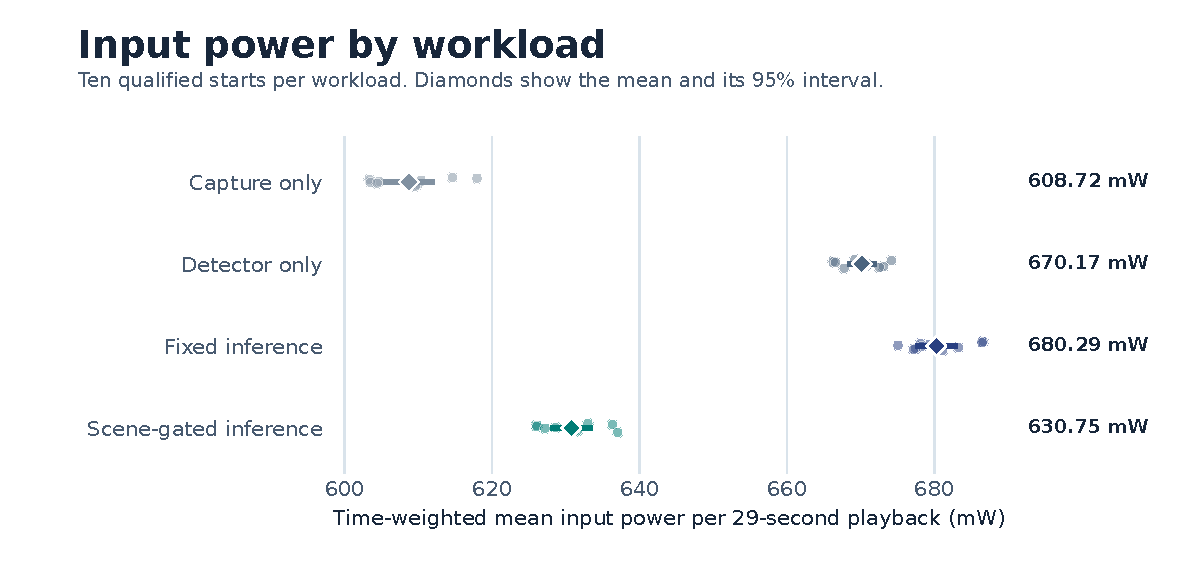
\includegraphics[width=\linewidth]{figures/02_workload_power.pdf}
\caption{Observed input power for ten windows per workload. Intervals describe marginal means. Figure~\ref{fig:pairs} accounts for the shared boot.}
\label{fig:workloads}
\end{figure}

\subsection{Coverage, delay and inference work}
Each full policy localized 30 of the 40 face episodes. The same three clip segments matched on all ten starts, and both modes missed the far-outdoor segment ten times. Median time to first match rose from 0.645 to 1.383\,s, a difference of 0.74\,s between the two conditional medians. Figure~\ref{fig:episodes} shows which episodes contribute to that comparison. It covers matched detections and does not assign a delay to missed episodes.

Detector calls fell from 498 to 160 (67.9\%) and embedding runs from 158 to 56 (64.6\%). All 214 embedding runs completed. Every matched face episode included qualifying crop coverage and completed model execution. Gating skipped detection on 579 stable-scene observations. Of its 160 detector calls, 103 were periodic and 57 were change-triggered; they produced 18 and 12 first matches, respectively. Their independent effects would require an ablation. Quiet intervals contained four fixed detections across two of 40 quiet episodes and one gated detection in one quiet episode.

\begin{figure*}[t]
\centering
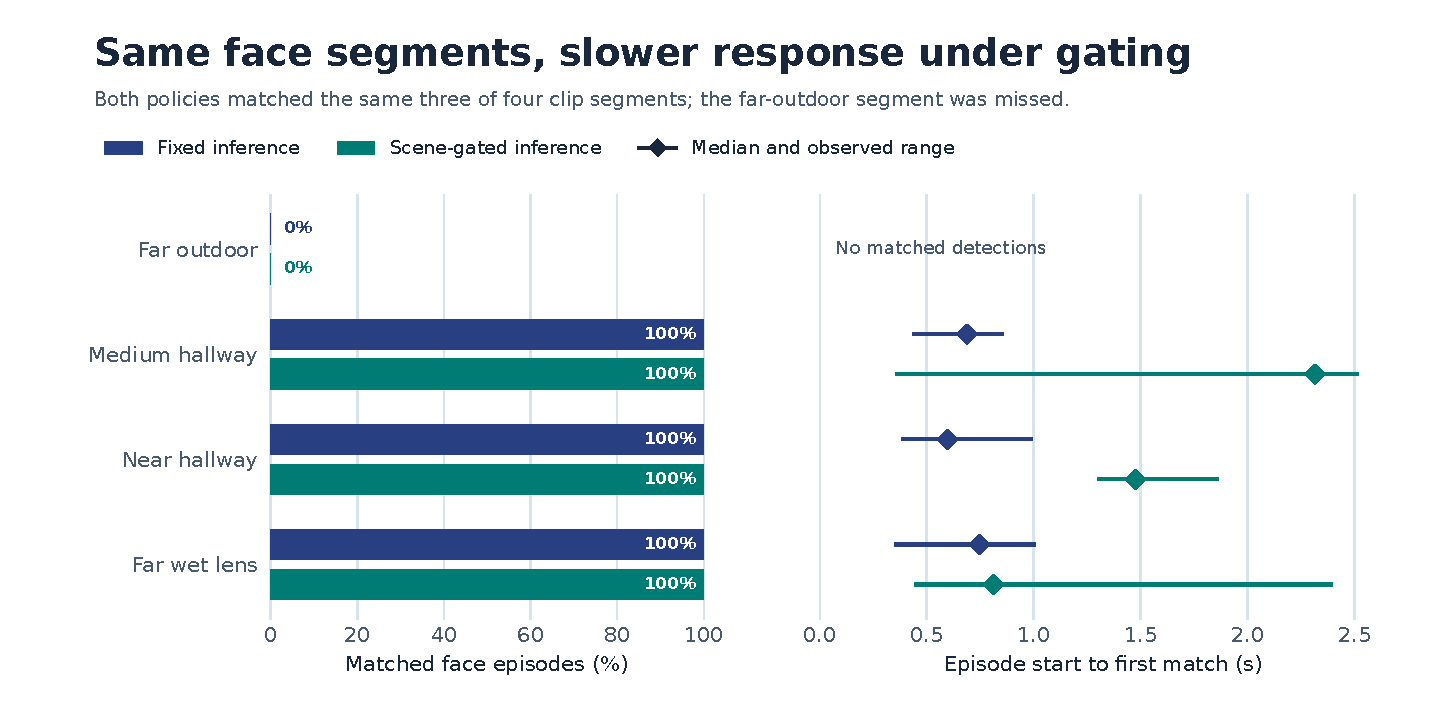
\includegraphics[width=0.75\textwidth]{figures/03_episode_coverage_latency.pdf}
\caption{Face coverage and time to first matched detection by clip segment. Each row aggregates ten replays of the same segment. Delay is conditional on matching. Both policies missed the far-outdoor segment on every replay.}
\label{fig:episodes}
\end{figure*}

\subsection{USB demonstration}
The functional test on the Mac displayed three public portraits across ten distinct presentations. The dashboard saved one image per presentation, zero images in eleven blank intervals, and no duplicate during a 40-second hold. All ten saved images matched the corresponding device observation by boot ID, frame ID, and hash. Within the observed phases, 411 of 413 preview JPEGs linked to results. This establishes local encounter capture for the tested presentation setup. Windows testing verified USB import and deduplication on existing board photos.

\subsection{Offline capture and battery}
A later USB-powered check closed the host serial connection. Two separated encounters produced two on-board photos; reconnection imported both with matching checksums, and a second import added none. Another screen rehearsal saved four photos across four encounters, with none added during a hold or five blank intervals. Manual gallery labels do not count as recognition. These checks verify host-disconnected capture and import; physical power-bank boot and battery life remain unverified.

\section{Separate host experiments}
\subsection{Recognition and face crop sensitivity}
The main recognition benchmark used SurvFace-derived \(96\times96\) grayscale crops. Olivetti was a separate 40-class sanity study \cite{olivetti}; LFW-derived portraits were used in historical screen-camera and crop-alignment diagnostics \cite{lfw}. These sources were not pooled into a single training or evaluation set. The main benchmark used five SurvFace identities seen in earlier development, 100 held-out known crops, and 300 held-out unknown crops from 50 other people. Each route used ten training roots (20261101--20261110) and its calibrated open-set rule on the same evaluation crops. Known image groups were separated across roles, but prior exposure to the roster limits generalization claims. Correct known acceptance requires accepting the crop and choosing its correct identity. Unknown false positive identification rate (FPIR) counts unknown crops assigned to any known identity. The compact INT8 gallery reached 3.5\% correct known acceptance and 4.2\% unknown FPIR. The larger INT8 classifier reached 4.6\% and 2.8\%, while its float counterpart reached 17.3\% and 3.3\% (Fig.~\ref{fig:recognition}). The roots share identities and evaluation crops, so their spread describes training variability.

The transfer models used Adam, cross-entropy, balanced batches of 24, a 64-unit ReLU embedding, and a six-logit head. Head training ran for up to six epochs at learning rates \(10^{-3}\) (\(\alpha=0.10\)) and \(5\times10^{-4}\) (\(\alpha=0.25\)); fine-tuning allowed 18 epochs at \(10^{-4}\), unfreezing the top 25\% and 50\%, respectively. The smaller route used no augmentation; the larger used the recorded mild grayscale augmentation. Stopping-role selection used patience three. INT8 conversion used up to 128 train-only representative crops; rejection thresholds were calibrated separately for each output backend before evaluation.

An earlier host diagnostic held MobileFaceNet fixed: FOMO-centered crops correctly accepted 4 of 15 known development groups, versus 14 of 15 with YuNet alignment. Galleries and calibration were crop-specific. This reused-data host comparison motivated checking localization separately; it does not measure Nicla recognition accuracy.

\begin{figure*}[t]
\centering
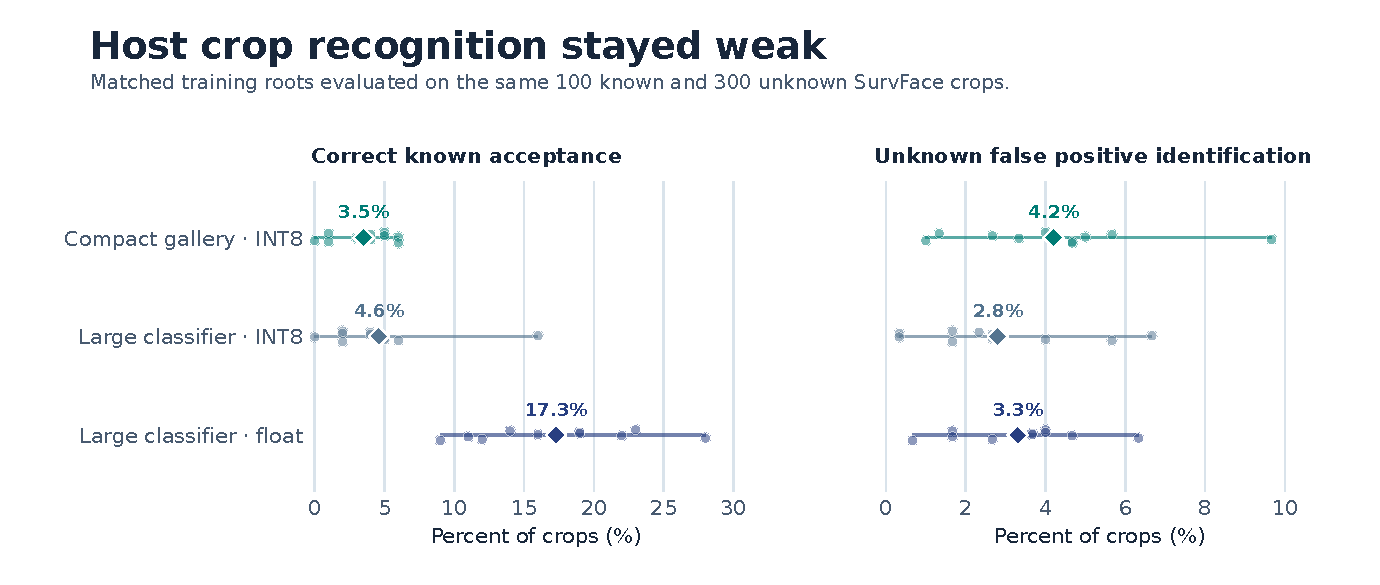
\includegraphics[width=0.72\textwidth]{figures/05_host_recognition.pdf}
\caption{Separate recognition experiments on held-out host crops. Each model route was run with ten initializations using the same evaluation set. These results motivated disabling known identity acceptance for the device demo.}
\label{fig:recognition}
\end{figure*}

\subsection{Model compression}
We compared 13 optimization arms over ten matched training initializations on a development workload. For the \(\alpha=0.25\) classifier, ordinary pruning and quantization-aware training (QAT) left the serialized INT8 file at 327{,}072 bytes in the tested export path. Physically removing channels reduced it to 280{,}248 bytes, a 14.3\% reduction (Fig.~\ref{fig:compression}). Estimated multiply--accumulates decreased by 303{,}104 while estimated peak activation memory stayed at 75{,}280 bytes. The channel-removal arm raised mean unknown FPIR from 3.2\% to 5.2\% on development crops. The benchmark concerns host exports and static estimates. The power study used the separately benchmarked compact gallery model.

\begin{figure}[t]
\centering
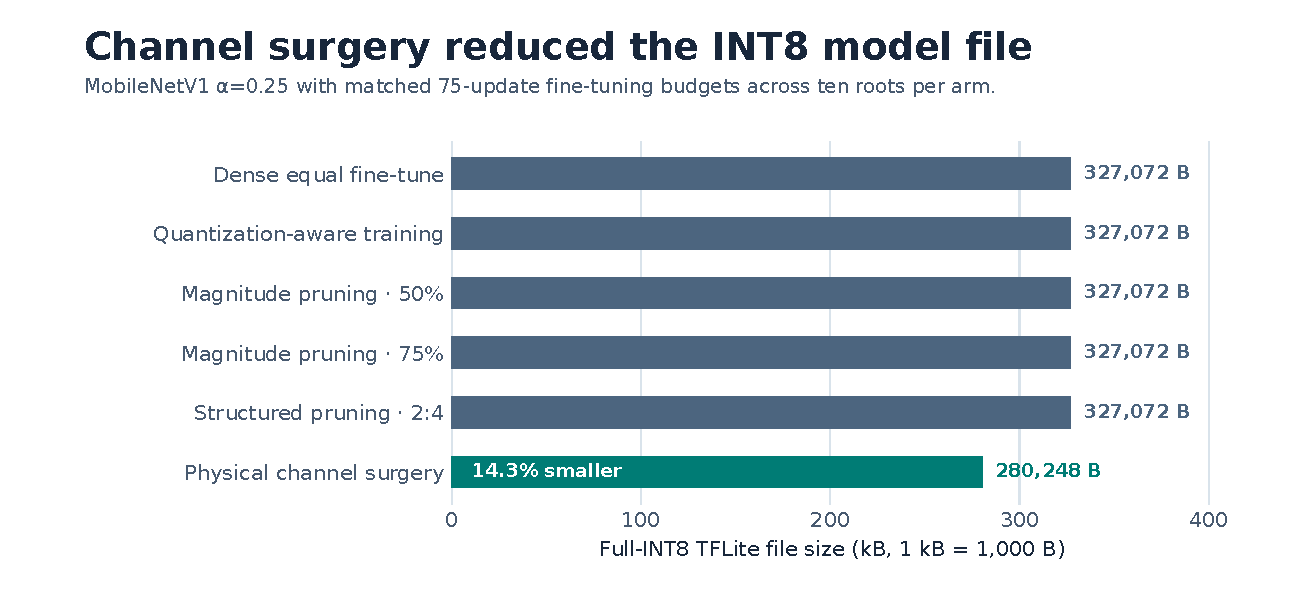
\includegraphics[width=\linewidth]{figures/06_compression_size.pdf}
\caption{INT8 file size under matched training budgets. The storage benefit came from physically changing tensor shapes in this export path. The comparison uses host development data.}
\label{fig:compression}
\end{figure}

\section{Discussion and limits}
The work avoided by gating was much larger than the percentage of board power saved. The capture-only control and the awake camera explain why the baseline matters. The periodic path ran more often than the change-triggered path. A shorter interval could improve response time but increase detector work, which makes the interval a useful parameter for a subsequent power versus delay sweep.

The pairing controls for the board boot within each block. Ten starts with one board, one meter, and one optical replay characterize a repeatable bench case. The repeated 40 episode observations per policy come from just four positive segments. Missing the far-outdoor segment under both policies points to a failure shared by the pipelines under those conditions. The study does not isolate distance from the other properties of that clip segment. A broader stress study would vary face size and duration across physically distinct scenes and measure field performance. Recognition generalization and battery life would require dedicated validation.

The FNIRSI had no independent calibration against a reference instrument. Native report anomalies contributed to exclusions. The paired interval describes between-block sampling variation for the accepted bench runs, and absolute instrument error or selection effects are outside that interval. USB input power includes the operating board and camera and is measured at the meter. The instrument and test topology can affect the reading. The recorded Edge Impulse feature checkpoints and host face references also have incomplete pretraining-corpus documentation. Their use cannot establish identity-disjoint pretraining or remove the screen-to-field domain gap.

\section{Conclusion}
On this clip, scene gating reduced USB input power by 7.28\% while matching the same face episodes, with 0.74\,s additional conditional median delay. The prototype also saved one image per verified portrait encounter. The result establishes a measured scheduling tradeoff on the Nicla; reliable known-person recognition and battery operation remain separate goals.

\section*{Reproducibility and artifacts}
The public \href{https://github.com/sophiayuanproj/FaceRecognition}{project repository} supplies firmware, dashboard, training and evaluation code, frozen manifests, and setup instructions. The \href{https://github.com/sophiayuanproj/FaceRecognition/releases/tag/research-assets-2026-11-22}{research-assets-2026-11-22 release} holds fitted checkpoints and raw power evidence. Measured firmware and model hashes are pinned in \texttt{bench/RELEASE\_HASHES.json}. \texttt{TRAINING.md}, \texttt{DATA.md}, and \texttt{evidence/README.md} cover training, original data provenance, and replay. Private camera recordings and original source images are excluded.

Run \texttt{python3 tools/fetch\_power\_evidence.py} from the checkout. It verifies the raw archive's full SHA-256 and 41{,}332{,}455-byte size. Extract it, enter its root, and run:
\par\noindent\begin{minipage}{\linewidth}
\begin{flushleft}\footnotesize\ttfamily
L=prior-results/final-block-ledger.csv\\
python3 resume/replay\_belkin\_primary.py \textbackslash\\
\hspace*{1em}-{}-runs resume -{}-schedule "\$L" -{}-expect-count 10
\end{flushleft}
\end{minipage}\par
Replay recovers ten paired starts, 40 windows, and a gated-minus-fixed mean of \(-0.04954\) W. The paper source includes plotting tables and the trigger and order audit.

{\footnotesize
\bibliographystyle{plain}
\bibliography{references}
}
\end{document}
